\documentclass{abnt}
%\usepackage[a4paper, inner=1.5cm, outer=2cm, top=3cm, bottom=2cm, bindingoffset=1cm]{geometry}
\usepackage[utf8]{inputenc}
\usepackage[english,brazilian]{babel}
\usepackage{rotating}
\usepackage{hyperref}
\usepackage{url}
\usepackage{indentfirst}
\hypersetup{%
    pdfborder = {0 0 0}
}
\usepackage{graphics}
\graphicspath{{./figuras/}}
\usepackage{placeins}
%\usepackage{lscape}
\usepackage{pdflscape}

\begin{document}

\autor{Rafael Tavares Amorim \par Rafhael Rodrigues Cunha\par Marcelo Maia Lopes }

\titulo{Redes e Sistemas Distribuídos: Trabalho Prático I}

%\orientador{Prof.}

\instituicao{Universidade Federal do Pampa \par Engenharia da Software}

\local{Alegrete - RS, Brasil}

\data{06 de Maio de 2012}

\capa

\folhaderosto

\tableofcontents


\chapter{INTRODUÇÃO}
Esse Documento tem por objetivo auxiliar o usuário no manuseio do chat, oferecendo ao mesmo um manual do usuário contendo manual de Instalação, configuração e utilização do software.

O documento também contem um manual de desenvolver, para fins de correção do trabalho e curiosidades, possuindo assim diagrama de classes, explicações sucintas sobre a linguagem que foi utilizada, e por fim uma introdução sobre o protocolo usado e o motivo pela escolha do mesmo.

\clearpage
\chapter{Manual do Usuário}

	\section{Instação}	
	Como apoio a instalação será enviado juntamente com o relatório os arquivos fontes do projeto e os arquivos já compilados (jar); Para instalar basta apenas copiar os arquivos jars (bate-papo-cliente.jar, bate-papo-servidor.jar) para a pasta desejada, abrir o terminal do seu sistema operacional, como exemplo utilizarei o windows, e fazer os seguintes procedimentos:
	\begin{enumerate}
	
	\item  Navegar ate a pasta aonde você copiou os jars, tanto o bate-papo-servidor quanto o bate-papo-cliente.
	Lembrando que para navegação utilizamos: 
	
	\begin{itemize}
	\item comando 'cd' - para abrir uma pasta;
	\item comando 'ls' - para visualizar o que esta dentro de uma pasta;
	\end{itemize}	
	
	\item Quando você chegar até a pasta aonde se encontra esses arquivos, digite java -jar nomedoarquivo.jar
	no nosso exemplo então ficaria da seguinte maneira:
	\begin{itemize}
	\item java - jar bate-papo-servidor.jar
	\end{itemize}
	Logo após darmos esse comando será inicializado o nosso servidor no qual receberá as mensagens do chat.
	
	\item Após, seguimos no terminal e dessa vez digitamos o seguinte comando: java -jar bate-papo-cliente.jar
	desse modo iniciaremos a interface gráfica na qual vai ser possível começar a utilização do chat.
	\end{enumerate}
	
	\section{Configuração}	
	Para se conectar ao servidor, deverá ser escrito na interface gráfica que abrimos anteriormente o comando (SERVER ip porta),onde o SERVER é o comando para conectar ao servidor,ip é o ip da maquina que se encontra o servidor inicializado (no nosso caso localhost) e porta seria a porta na qual o servidor esta configurado para ser utilizado no caso (8080). 
	após este comando, você deverá receber a mensagem do servidor de boas vindas. 	

	Finalizando essa primeira etapa, passamos a etapa de configuração do nosso nickname (o apelido que utilizaremos para interagir com os demais participantes do chat), para isso digitaremos o seguinte comando:
	\begin{itemize}
		\item USER nome	
	\end{itemize}
	onde USER é o comando para especificar que gostaria de mudar de nick e nome é o nome no qual escolhi.

	Possiveis problemas que podem aparecer:
	\begin{enumerate}
		
		\item  OK\_USERNAME caso o nome seja aceito
		\item  ERR\_INVALIDUSERNAME caso o nome do usuario seja invalido
		\item  ERR\_NEEDMOREPARAMS caso você não tenha digitado o nome
		\item  ERR\_ALREADYREGISTRED caso o nome digitado já esteja na lista	
	\end{enumerate}
	
	\section{Utilização}		
	Após terminarmos a instalação e configuração do nosso chat, agora iremos utiliza-lo o mesmo. A utilização assim como as outras etapas é bem simples e consiste em mandar/receber mensagens.
	Então, partindo para o pratico, para enviarmos uma mensagem para outra pessoa no modo normal, ou seja, todos os demais participantes do chat tambem verão essa mensagem digitamos o seguinte comando:
	\begin{itemize}
		MSG mensagem 	
	\end{itemize}
	onde MSG é meu comando que indica que estarei escrevendo uma mensagem e a 'mensagem' é o que eu gostaria de digitar, exemplo: MSG oi.
	Após digitar esse comando sua mensagem será enviada a todos os demais utilizadores do chat naquele momento.
	
	Além dessa possibilidade ainda podemos enviar mensagens privadas (mensagens entregues somente ao usuario desejado), para isso utilizaremos o seguinte comando:
	\begin{itemize}
		PRIVMSG username_destino mensagem
	\end{itemize}
	Onde PRIVMSG indica que quero enviar uma mensagem do tipo privada, username_destino é o nick do usuário no qual eu gostaria de enviar a mensagem e mensagem é a minha mensagem propriamente dita.


\clearpage
\chapter{Manual do Desenvolvedor}
	\section{Diagrama de Classes}	
	
	\begin{figure}[htp]
		\begin{center}
			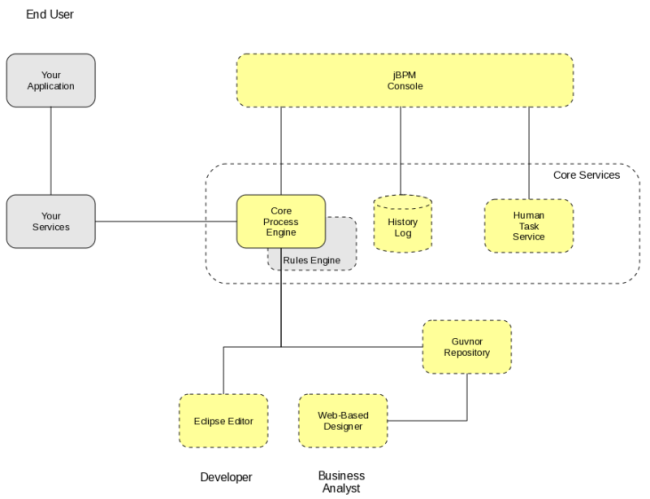
\includegraphics[width=300px]{jbpm_overview}
			\caption{Diagrama de Classes}
			\label{fig:jbpmOverview}
		\end{center}
	\end{figure}
	\FloatBarrier
	
	\section{Linguagem Utilizada}	
		A linguagem utilizada de apoio para desenvolvimento da solução do trabalho proposto foi o java, porque alem de ele ser multiplataforma, ou seja, rodar em diversos sistemas operacionais ele também possui muitos tratamentos na parte de sockets que é uma classe utilizada na implementação da solução que facilita na parte de comunicação entre um cliente e outro.
	
	\section{Protocolo}		
		O protocolo escolhido para ser implementado foi o TCP/IP pois ele é um protocolo confiável, ou seja, as mensagens do chat não serão perdidas embora possam demorar um certo tempo para chegar, alem de possuir controle de fluxo e sequenciamento das mensagens.



\clearpage
%Referências Bibliograficas
\nocite{*}
\bibliographystyle{plain}		
\bibliography{bibliografia}		
\end{document}